%!TeX root=MemoriaTFG.tex
\chapter{Análisis de los datos \ac{GPS}} 
Con el fin de llevar a cabo una simulación de trayectorias, se tiene que realizar previamente
un análisis del territorio a simular. El análisis determinará parámetros de simulación que 
harán posible una generación de trayectorias semejantes a las reales. En este capítulo 
se explica como está estructurado este análisis. Se observará la importación de los datos
del territorio geográfico y del modelo lógico del terreno. Se explica el proceso de 
map-matching y su implementación con el algoritmo de Viterbi para la detección de los 
puntos. Finalmente, con el modelo de detección de puntos definido, se explica qué 
datos se van a explotar y de qué forma.


\section{Preparación del entorno de datos}
El entorno de datos con el que se trabaja dentro de la propuesta de este documento 
consta de dos partes fundamentales: los ficheros de trayectorias reales en formato
\ac{GPX} y el modelo lógico de carreteras y caminos por el que estos ficheros 
se sitúan. Durante esta sección se describen ambos.

\subsection{Importación de datos GPS a \textit{TrackSimulator}}
\label{section: ImportacionGPX}
%Importación de los datos gpx
Para realizar un tratamiento de los datos a partir de un fichero GPX se realiza un uso de la 
librería \textit{gpxpy}, cuya funcionalidad ha sido explicada anteriormente en el subapartado 
\ref{subsection: LibreriasExternas}. El primer paso a realizar es el parseo del fichero. 
La palabra parseo es un vocablo adaptado del inglés (parsing) con el que se describe el proceso 
de análisis de código, normalmente XML para obtener y tratar la información que contienen.
De esta forma encontramos un objeto \textit{track}, que contiene \textit{segments} que a su vez 
contienen los diferentes \textit{waypoints}. De esta
forma se obtiene la estructura que podemos ver en la figura \ref{figure: WayPointStructure} :

\begin{figure}[htb]
\begin{center}
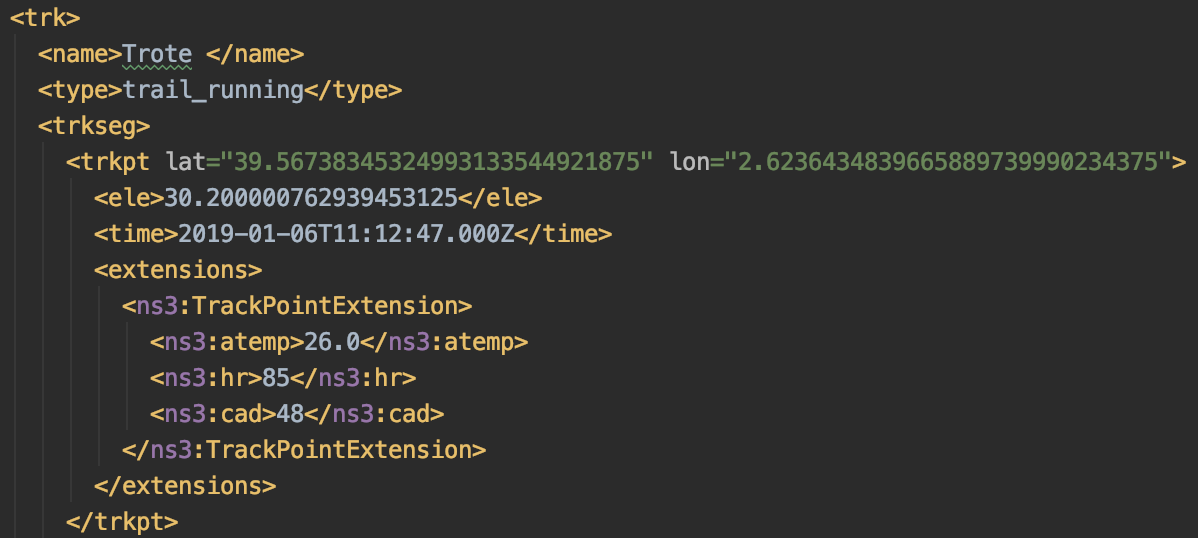
\includegraphics[width=0.9\textwidth]{./Imagenes/WayPointStructure.png}
\caption{Estructura de un \textit{track} dentro de un fichero .\ac{GPX}}
\label{figure: WayPointStructure}
\end{center}
\end{figure}
\newpage
La información necesaria para la implementación de la solución propuesta en este documento es 
la posición en latitud y longitud de cada uno de los puntos. El tiempo  y la elevación han quedado fuera 
del alcance de esta propuesta. El resto de información tanto de puntos (elevación) como de segmentos 
(metadatos) no será usada para el desarrollo de la propuesta, queda una estructura en forma de lista del 
siguiente tipo 
de elemento.
\begin{table}[h]
\centering
\begin{tabular}{l | c | l} 
\toprule
\multicolumn{3}{c}{\textbf{Punto preprocesado}} \\ 
\cmidrule(r){1-3}
{\textbf{Campo}} &  {\textbf{Tipo}} & {\textbf{Descripción}} \\
\cmidrule(r){1-3}
{longitud}  & Float & Posición del nodo respecto al eje horizontal. \\
{latitud}  & Float & Posición del nodo respecto al eje vertical.\\
\bottomrule
\end{tabular}
\caption{Estructura lista de puntos.}
\label{TablaNodo}
\end{table}
\newpage
Se ha decido realizar de esta forma para facilitar la manejabilidad de los datos mediante el objeto 
\textit{TrackPoint}, que es un objeto nexo a toda la funcionalidad del aplicativo. 

\subsection{Entidad TrackPoint}
Para añadir una capa de abstracción adicional al aplicativo toda interacción dentro del sistema se 
realiza a partir de la entidad TrackPoint. Esta entidad es una clase que extiende de la clase Point 
de la librería shapely, de esta forma, nos aseguramos que si en un futuro la librería externa deja de 
funcionar podremos extender otra clase usable, siempre implementando los métodos necesarios 
asimismo,tenemos una entidad lógica que puede ser ampliada en futuras iteraciones del 
aplicativo.

\subsection{Importación de caminos y carreteras al modelo de datos}
\label{section: EstructuraLogica}
%Obtención del grafo
En esta propuesta se ha optado por plantear la solución de importación usando una red compleja, siguiendo el modelo establecido por G.Boeing [14]. Para abordar correctamente la 
problemática del análisis de rutas dentro del espacio urbano se debe plantear una solución con 
una red compleja. 
Esta red está modelada en forma de grafo. Con esta estructura de datos se puede contemplar un 
proceso de importación, análisis, y exportación de datos geográficos. Para realizar la importación 
de los datos se recurre a la librería OSMnx comentada en la subsección \ref{subsection: 
LibreriasExternas}. Mediante el uso de un corto número de instrucciones se consigue importar 
toda la estructura de la zona del Castell de Bellver.
\begin{lstlisting}[caption={Importación de una zona mediante la librería osmnx.}\label{algoritmo:graphFromBbox}, language=Python] 
	self.graph = osmnx.graph_from_bbox(north, south, east, west)
\end{lstlisting}


%Traramiento de la estructura
Con la importación de los datos se ha conseguido obtener la información de OpenStreetMap, 
no obstante se debe realizar un tratamiento de filtrado de los datos importados debido a que 
aparece información que en este proyecto no tienen relevancia. Esta información se trata de 
características concretas de calles, peatonales o no, como la dirección. Nuestro planteamiento del 
problema define que la trayectoria a simular no tiene en cuenta el sentido de la carretera. Eso 
quiere decir que una carretera para vehículos de una dirección, se convierte en un camino de 
posible transito. 

Por otra parte, se añade información tanto a los nodos como a las aristas del grafo para 
almacenar información necesaria para la solución del problema. Por lo tanto, al final del tratamiento 
de la red obtendremos un grafo dirigido, donde las intersecciones entre la infraestructura urbana (
calle, camino, carretera) están definidas como un nodo y la característica de esta como la arista. Por 
simplicidad de entendimiento para la implementación de soluciones se ha decidido aplicar dos 
aristas por cada nodo en común, con la información geoespacial correspondiente. La red 
compleja queda establecida como muestran las tablas \ref{TablaNodo} y \ref{TablaArista} una vez aplicado el procesado:
\begin{table}[h]
\centering
\begin{tabular}{l | c | l} 
\toprule
\multicolumn{3}{c}{\textbf{Nodo}} \\ 
\cmidrule(r){1-3}
{\textbf{Campo}} &  {\textbf{Tipo}} & {\textbf{Descripción}} \\
\cmidrule(r){1-3}
{Identificador}  & Integer  & Clave del nodo.\\
%\cmidrule(r){1-2}
{x}  & Float & Posición del nodo respecto al eje horizontal. \\
{y}  & Float & Posición del nodo respecto al eje vertical.\\
{osmid} & Integer & Identificador de \ac{OSM} \\
\bottomrule
\end{tabular}
\caption{Estructura nodo.}
\label{TablaNodo}
\end{table}
\begin{table}[h]
\centering
\begin{tabular}{l | c | c } 
\toprule
\multicolumn{2}{r}{\textbf{Arista}} \\ 
\cmidrule(r){1-3}
{\textbf{Campo}} &  {\textbf{Tipo}} & {\textbf{Descripción}} \\
\cmidrule(r){1-3}
{Identificador}  & (Integer, Integer, Integer)  & {Clave de la arista}\\
%\cmidrule(r){1-2}
{osmid}  & Integer  & Identificador de \ac{OSM} \\
{oneway} &  Boolean & Carretera de un único sentido. \\
{name} & String & Nombre de la carretera. \\
{highway} & String & Tipo de carretera. \\
{length} & Float & Longitud del camino. \\
{geometry} & LineString & Geometría de la carretera. \\
{num of detections} & Integer & Núm. de detecciones de puntos. \\
{frequency} & Float & Frecuencia de puntos detectados. \\
\bottomrule
\end{tabular}
\caption{Estructura arista.}
\label{TablaArista}
\end{table}
\newpage

\section{Map-Matching}\label{section: MapMatching}
Uno de los grandes retos del análisis de trayectorias es la identificación y asignación de cada uno de los puntos GPS en su correspondiente trayectoria. Este proceso es llamado Map-Matching. Los puntos GPS se obtienen a partir de un dispositivo que administra la serie de puntos GPS correspondientes a una trayectoria con un cierto error o desviación. Esta serie de puntos son puntos aislados y no tienen relación directa con el modelo lógico establecido, es decir, con la información geográfica asociada.

Existen diversos procedimientos para abordar el problema del \textit{Map-matching}. La 
aproximación al problema en esta propuesta se realiza aplicando el modelo probabilístico de las 
cadenas de Markov, que explicamos en el siguiente apartado.

\subsection{Hidden Markov Model (\ac{HMM})}
%Explicar que es una cardena de Markov
\ac{HMM} sigue el modelo estadístico tradicional de Markov \cite{Malvar08}. En 1907, A. A. Markov 
comenzó el estudio de un proceso donde un experimento podía afectar a la salida del siguiente 
experimento. Este tipo de proceso se denominó Cadena de Markov. 
%https://www.dartmouth.edu/~chance/teaching_aids/books_articles/probability_book/Chapter11.pdf

Definiremos un conjunto de estados $ S = {s_{1}, s_{2}, . . . , s_{n}}. $ El proceso empieza en un estado inicial y se traslada de estado en estado. Esta transición se le denomina \textit{step}. Los \textit{steps} entre un estado $S_{i}$  y $S_{j}$ cumple una \textbf{probabilidad de transición}.

Por otro lado encontramos la \textbf{probabilidad de emisión}. Esta probabilidad responde a observar un estado $S$ en un instante $t$ determinado.

Markov define como suposición de primer orden que la probabilidad de ocurrencia de un evento en un tiempo $t$ solo dependerá de $t-1$. De esta forma las observaciones ${O-2,..., O-n}$ no 
afectaran directamente a $t$.

%(https://buildmedia.readthedocs.org/media/pdf/hidden-markov/latest/hidden-markov.pdf)
\subsection{Aproximación de Hidden Markov Model a Map-matching}
La estructura lógica del territorio en esta propuesta está definida como un grafo formado por diferentes \textit{nodos} y \textit{aristas}. Los nodos corresponden a la intersección entre caminos, mientras que en las aristas se almacena la información referente a la constitución geográfica de estos.

Esta información queda almacenada en un \textit{Shape} de forma que se trata de una sucesión de puntos \ac{GPS} tal y como se muestra en la siguiente imagen:
\begin{figure}[htb]
\begin{center}
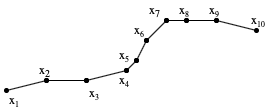
\includegraphics[width=0.6\textwidth]{./Imagenes/LineString.png}
\caption{Ejemplo de estructura LineString}
\label{figure: LineString}
\end{center}
\end{figure}

Cada uno de las proyecciones sobre los subsegmentos identificados entre $x_{1}, ..., x_{10}$ son proyecciones validas a una observación determinada.

Por otra parte aparece la información \ac{GPX}. El fichero que almacena la información de trayectorias que se han realizado en las delimitaciones de nuestro territorio. Esta serie de puntos se identifican como \textbf{observaciones}. Tenemos entonces los dos elementos principales que se han descrito anteriormente: una serie de observaciones y un modelo. A partir de aquí, se plantea el \textbf{problema general de decodificación}: dada una secuencia de observaciones, ¿qué secuencia de estados es la más probable para generarlos?
Este problema se resuelve mediante la implementación del \textbf{\textit{Algoritmo de Viterbi}}, que explicamos a continuación.

\subsection{Algoritmo de Viterbi}
El algoritmo de Viterbi se presenta como una técnica computacional con la que se obtiene la 
sucesión de nodos más probable para una cadena de Markov. Para cada una de las proyecciones 
se obtiene una probabilidad, siendo la más alta la elegida para ser el nuevo elemento del camino de 
Viterbi. La figura \ref{figure: MapMatching} muestra el objetivo de este algoritmo, poder detectar que la secuencia de puntos corresponde a la trayectoria formada por los puntos $x_{n}$.

\begin{figure}[htb]
\begin{center}
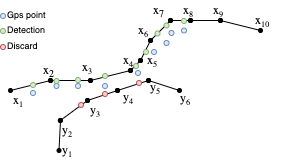
\includegraphics[width=0.6\textwidth]{./Imagenes/Map-matching.png}
\caption{Ejemplo teórico de detección map-matching mediante algoritmo de Viterbi}
\label{figure: MapMatching}
\end{center}
\end{figure}
\newpage

La probabilidad tiene en cuenta dos factores:
\begin{description}
\item [Probabilidad de emisión] Esta probabilidad es calculada por análisis espacial. Por convenio 
establecemos que cuanto más próxima sea la observación a la proyección más probable será que 
sea la elección correcta, partiendo de una distribución normal con media cero tal y como se 
muestra en la referencia \cite{HMM01}.
\begin{equation}
P_{emission}=\frac{1}{\sqrt{2\pi}\sigma}e^{-\frac{(d_{i}^{j}-\mu)^{2}}{2\sigma^{2}}} 
\end{equation}

\item [Probabilidad de transición] La probabilidad de llegar al estado $S_{i}$ de una proyección 
viene determinado por el estado anterior $S_{i-1}$ en una relación de dos aspectos. Por una parte 
la distancia espacial entre el  $S_{i}$ y $S_{i-1}$ identificado como $d(S_{i},S_{i-1})$. Por otra 
parte encontramos el camino más corto entre estos dos estados. El camino más corto definido 
como $SP(S_{i},S_{i-1})$ se entiende como la cantidad de nodos que se tienen que atravesar para 
llegar de  $S_{i}$ a $S_{i-1}$. Esta última se mantiene como una distribución exponencial de forma 
que a mayor número de nodos por atravesar en el camino más corto esta proyección es 
penalizada \cite{HMM01}..
\begin{equation} 
P_{transition}=\frac{distance(p_{i-1}, p_{i})}{e^{SP(p_{i-1}, p_{i})}}
\end{equation}
\end{description}

Los valores de $\sigma$ y $\beta$ se han obtenido mediante pruebas. Se observa en la figura \ref{figure:EmissionProb} la representación de la función de probabilidad de emisión respecto al valor de $\alpha$. Se ha escogido $\sigma = 4$ debido a que es un valor que da unos valores de 
probabilidad válidos para el rango de 5 a 10 metros. 

\begin{figure}[!htb]
\begin{minipage}{0.46\textwidth}
\centering
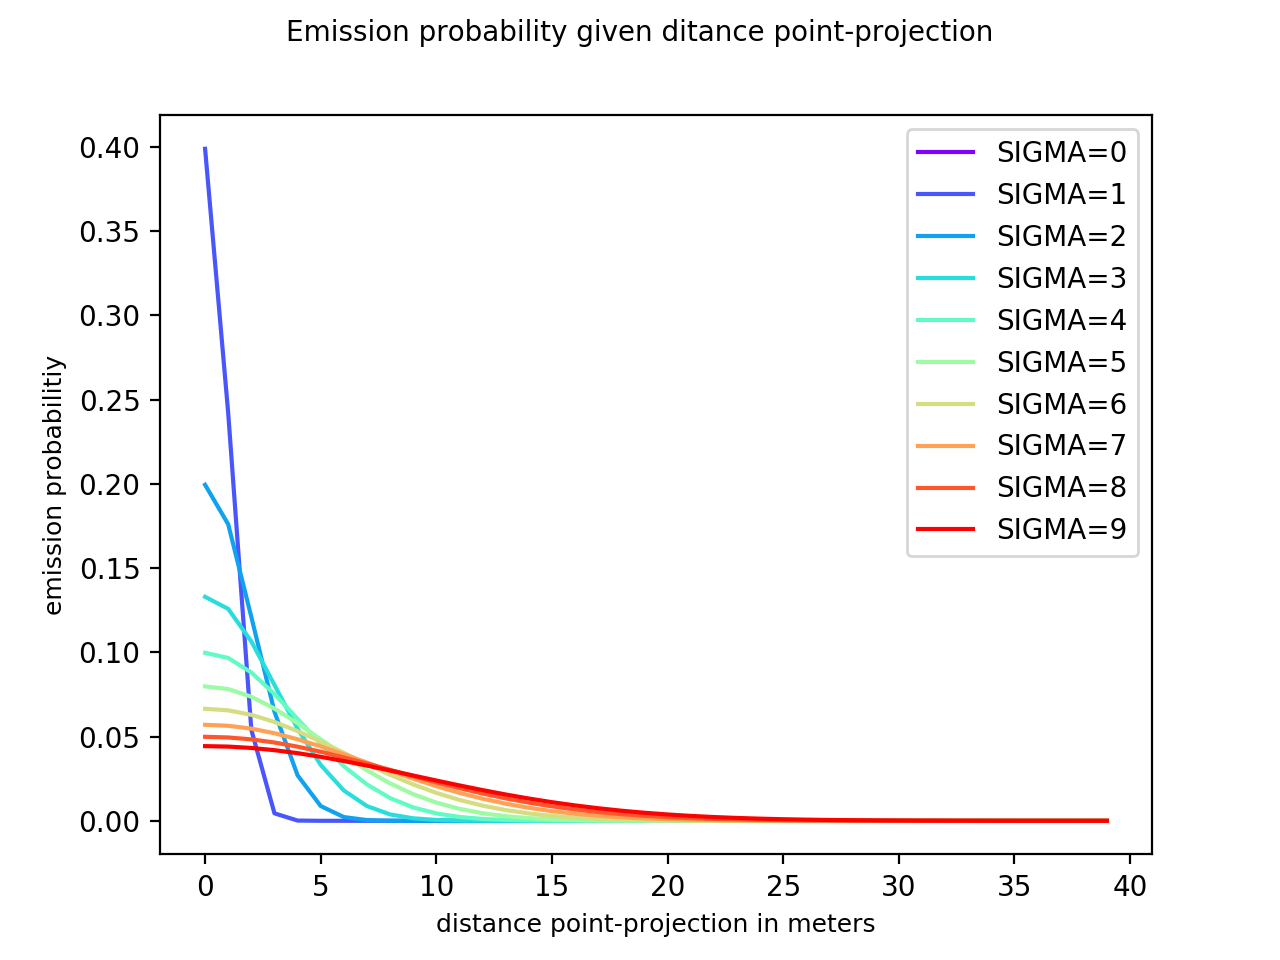
\includegraphics[width=1.2\textwidth]{./Imagenes/EmissionProb.png}
\caption{Análisis de la función de $P_{emission}$ para $\sigma$.}
\label{figure:EmissionProb}
\end{minipage}\hfill
\begin{minipage}{0.46\textwidth}
\centering
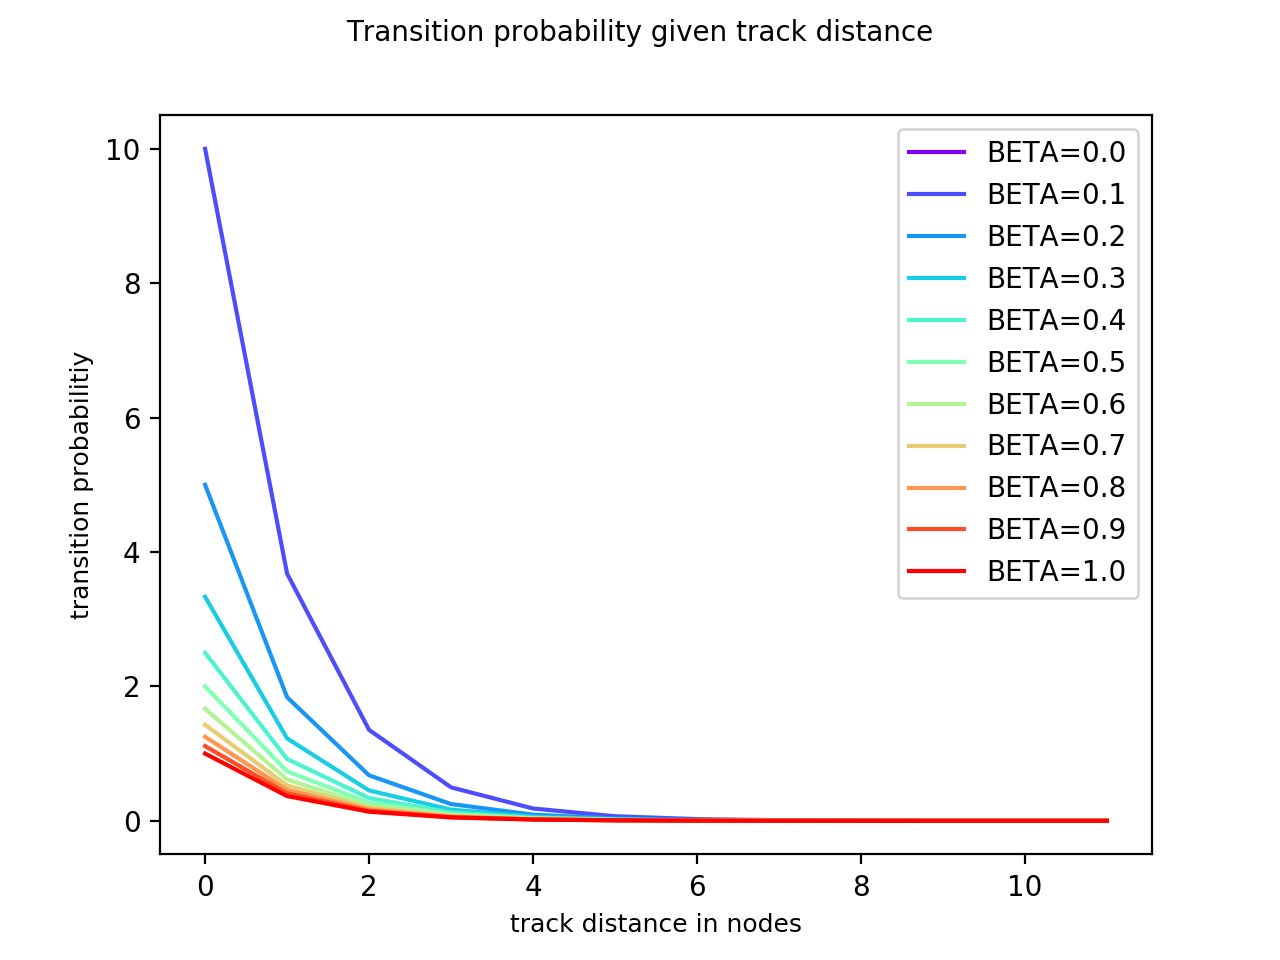
\includegraphics[width=1.2\textwidth]{./Imagenes/TransitionProb.png}
\caption{Análisis de la $P_{transition}$ de transición para $\beta$.}
\label{figure:TransitionProb}
\end{minipage}
\end{figure}

Por otro lado, la figura \ref{figure:TransitionProb} es la representación de la probabilidad de 
transición respecto a $\beta$. Se ha determinado que $\beta = 0.1$ porque la 
probabilidad de transición es adecuada debido a que es tolerante con valores entre 1 y 3 nodos de 
distancia, y para los datos tratados ofrece valores válidos. Cabe destacar que estos valores son 
modificables según la exactitud con la que cuenten los datos.


La implementación del algoritmo se realiza de forma iterativa para todos los puntos \ac{GPS} de la 
trayectoria. Por cada punto se buscan las proyecciones en un radio determinado. De esta forma se 
realiza una primera criba de proyecciones que no serán probables.
Por cada una de las proyecciones se calcula las probabilidades descritas anteriormente. La 
probabilidad de transición viene determinada por el estado anterior, tal y como se puede observar en 
la fórmula. Una vez tratadas todas las proyecciones. Se almacena aquella proyección con la mayor 
probabilidad total. Si el camino más corto entre el nodo correspondiente a la proyección $p_{i}$ y 
$p_{i-1}$ es mayor que uno se debe completar el camino más corto. 

Con la aplicación de esta información se obtiene una secuencia de puntos \ac{GPS} relacionados 
con la estructura de datos y queda solucionado el problema del \textit{map-matching}.

\subsection{Ejemplo de aplicación del algoritmo de Viterbi}
Con el siguiente ejemplo se pueden observar los beneficios y los inconvenientes de la aplicación del algoritmo 
implementado en esta propuesta.

En la figura \ref{figure:MapMatching1} se observa en puntos rojos la trayectoria real de un individuo dentro del 
territorio limitado del Castell de Bellver. Los puntos verdes corresponden a la detección de las proyecciones 
más probables por parte del algoritmo de Map-matching.

\begin{figure}[htb]
\begin{center}
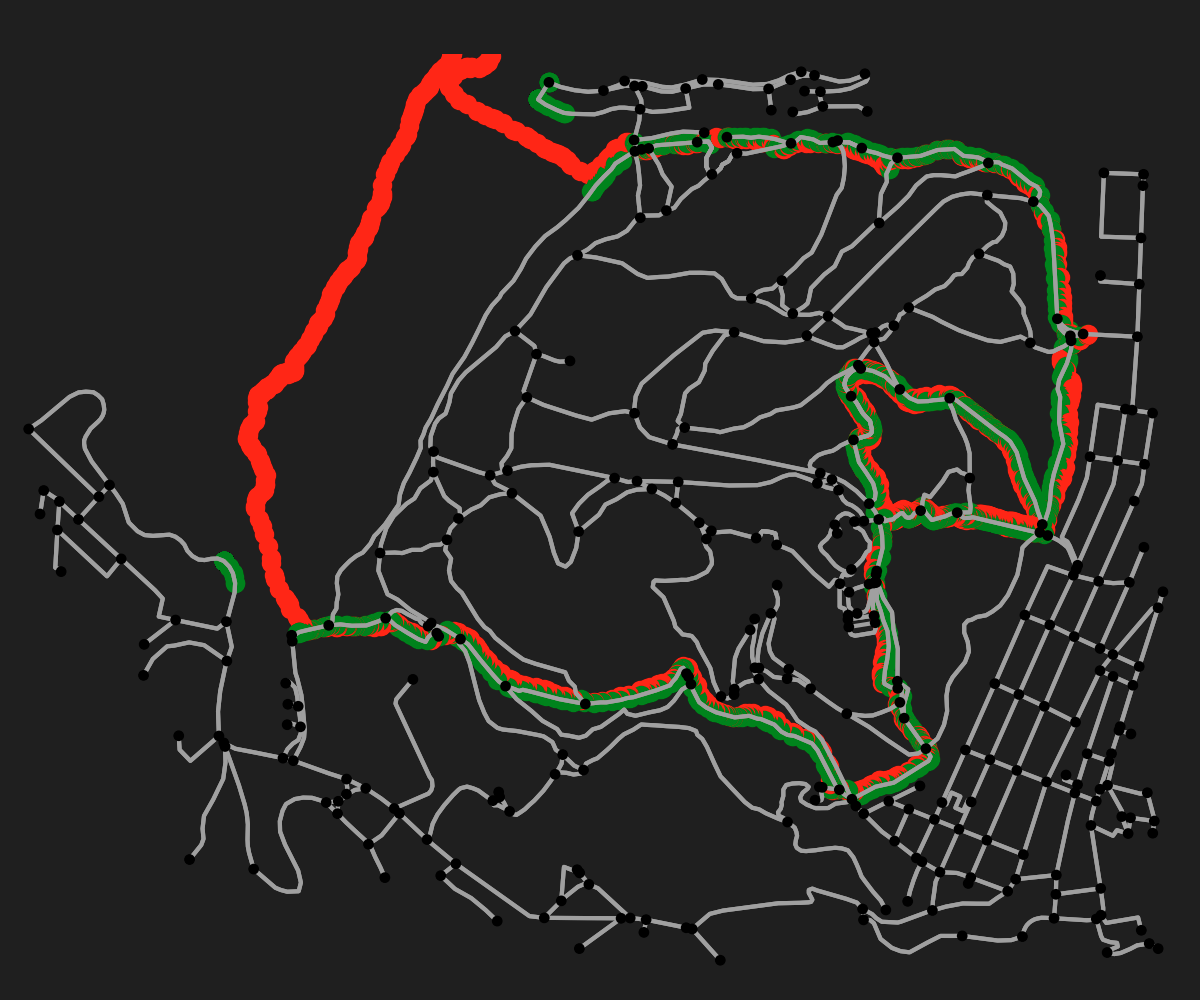
\includegraphics[width=0.6\textwidth]{./Imagenes/MapMatching1.png}
\caption{Ejemplo de aplicación de algortimo de Viterbi para detección de trayectorias.}
\label{figure:MapMatching1}
\end{center}
\end{figure}

El algoritmo realiza una detección punto a punto de su proyección dentro del camino. Pueden 
aparecer situaciones en las que por desviación de precisión en la detección \ac{GPS} un punto parezca 
situarse cerca de un camino no correcto. No obstante, la probabilidad de transición descrita en 
el apartado anterior se encarga de ofrecer como opción más probable, aquella donde el 
\textit{shortest path} del grafo sea menor. \ref{figure:GoodDetection}
\begin{figure}[htb]
\begin{center}
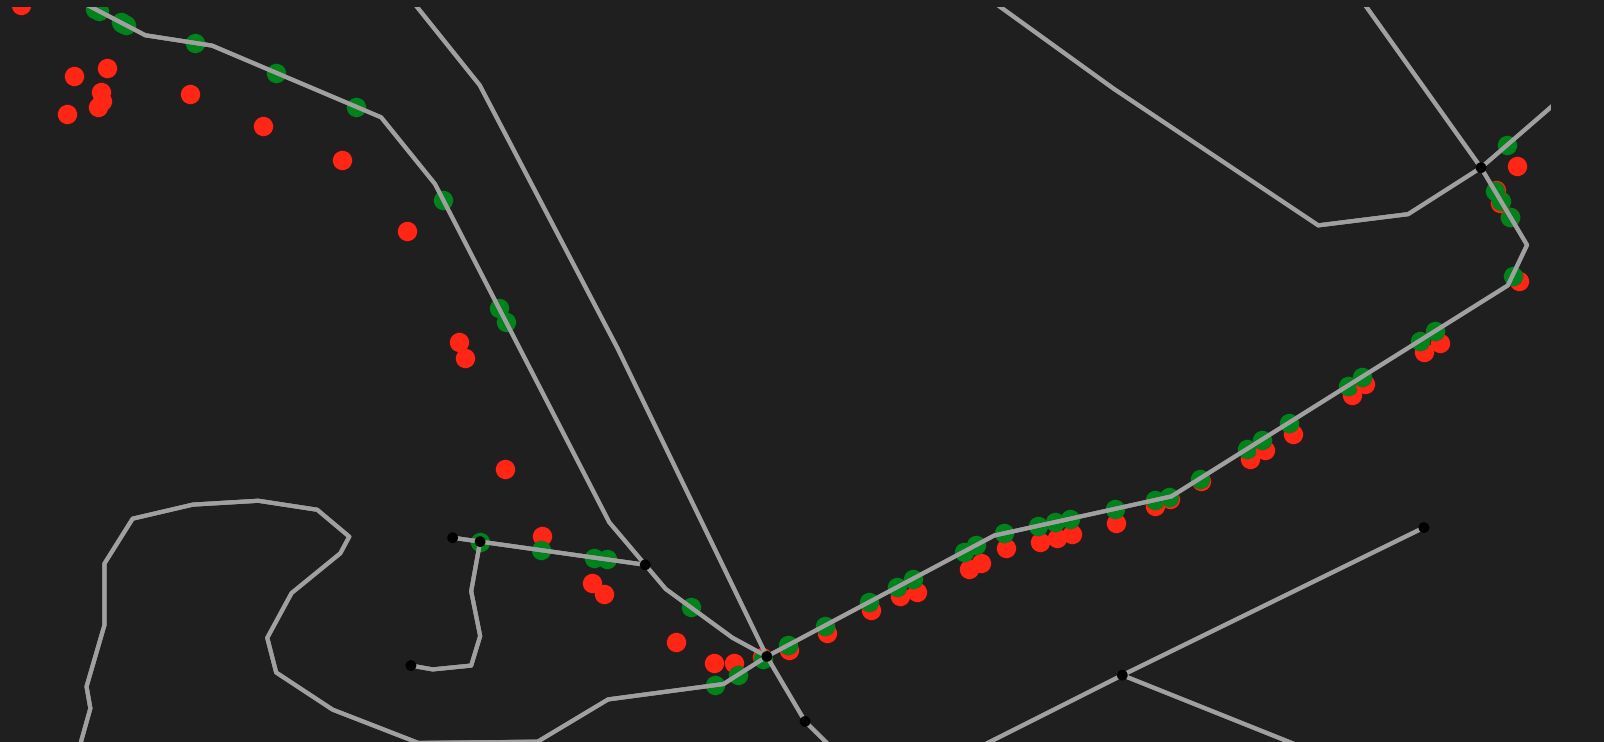
\includegraphics[width=0.6\textwidth]{./Imagenes/BuenaDeteccion.png}
\caption{Ejemplo de aplicación de algortimo de Viterbi para detección de trayectorias.}
\label{figure:GoodDetection}
\end{center}
\end{figure}
\newpage
No obstante pueden aparecer casos aislados donde la deteccion \ac{GPS} es tan cercana a una 
proyección de un camino incorrecto que hace imposible su no elección respecto a la proyección 
correcta. \ref{figure:BadDetection}
\begin{figure}[htb]
\begin{center}
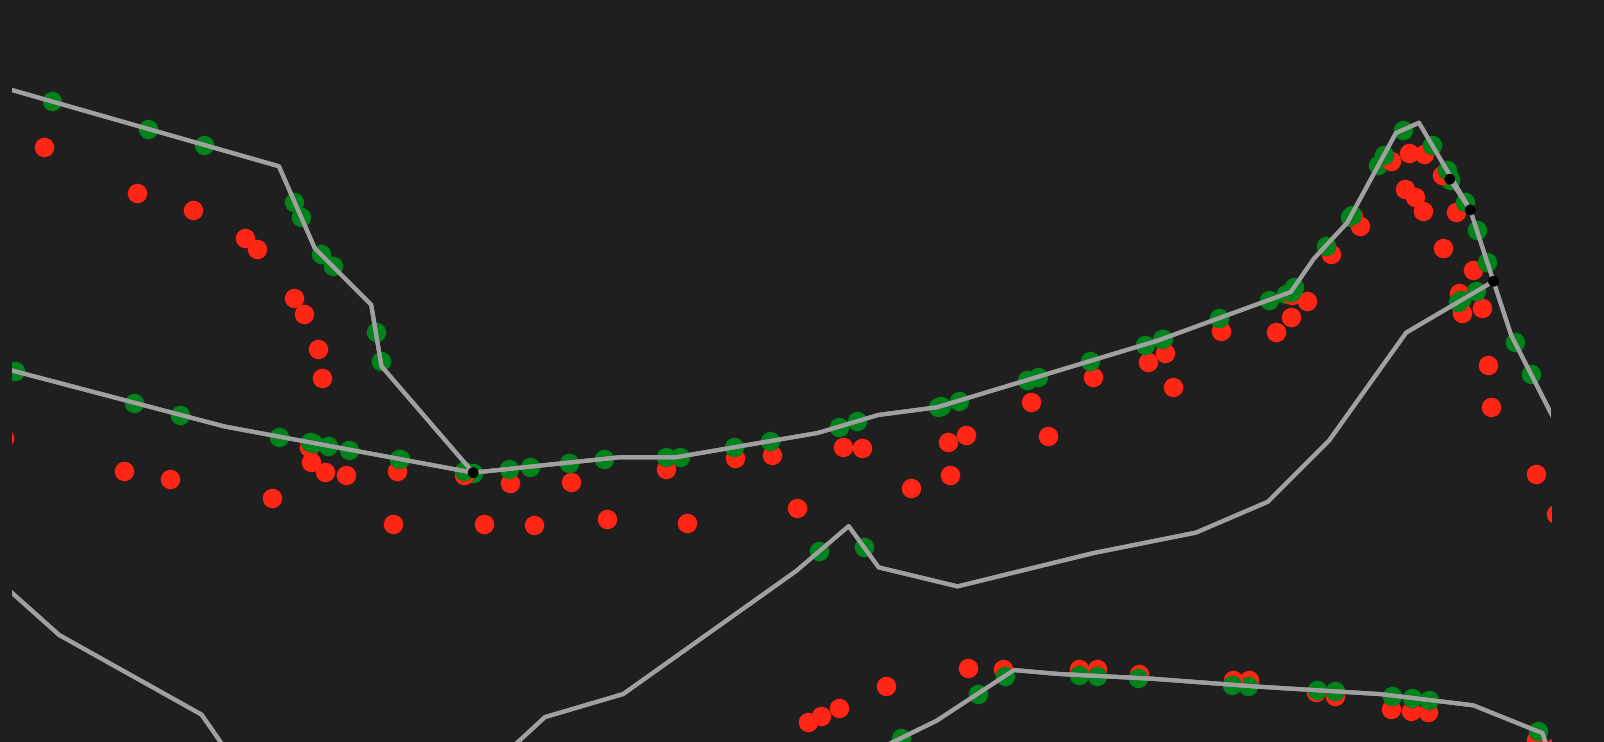
\includegraphics[width=0.6\textwidth]{./Imagenes/MalaDeteccion.png}
\caption{Ejemplo de aplicación de algortimo de Viterbi para detección de trayectorias.}
\label{figure:BadDetection}
\end{center}
\end{figure}
\newpage
Cabe destacar que el funcionamiento correcto de la detección de proyecciones depende de que el 
individuo realice el recorrido basado en los caminos posibles por el modelo de datos obtenido de \ac{OSM}. 
La detección de puntos por senderos no determinados previamente no pertenece al alcance de este problema.




\subsection{Implementación de Map-matching}
La implementación del algoritmo de map-matching se basa en dos grandes partes: 
el \textbf{\textit{Interactor}} \textit{get\_map\_matching} y la \textbf{\textit{Entity}} 
\textit{hidden\_markov\_model}

El primero de ellos, \textit{get\_map\_matching}, se trata de una interfaz cuya única responsabilidad 
consiste en realizar el proceso de detección de proyecciones descrito en apartados anteriores. La 
interfaz se mantiene abstracta a la utilización de cualquier otro método que no sea el camino de 
Viterbi. Es en la implementación de esta interfaz (\textit{get\_map\_matching\_impl} la que almacena 
la lógica. En la implementación propuesta despliega el método \textit{viterbi\_algorithm} de la 
entidad \textit{hidden\_markov\_model}.

\begin{lstlisting}[caption={Implementación interactor get\_map\_matching\_impl}\label{algoritmo:MapMatchingImpl},language=Python] 
class GetMapMatchingImpl(GetMapMatching):
    def __init__(self, detection_model: HiddenMarkovModel):
        self.detection_model = detection_model

    def match(self, points):
        mapped_track, _ = self.detection_model.viterbi_algorithm(points)
        return mapped_track
\end{lstlisting}

Por otra parte, encontramos \textit{hidden\_markov\_model}. Se trata de una entidad abstracta que 
almacena los métodos necesarios para implementar la detección de proyecciones. Los métodos 
necesarios para implementar una cadena de Markov son los cálculos de probabilidad de emisión y 
de probablidad de transición. Éstos junto con la implementación del algoritmo de Viterbi describen 
toda la responsabilidad de esta entidad.

\begin{lstlisting}[caption={Declaración interfaz hidden\_markov\_model}\label{algoritmo:HiddenMarkovModel},language=Python] 
class HiddenMarkovModel(abc.ABC):
    @abc.abstractmethod
    def get_emission_prob(self, projection, point):
        pass

    @abc.abstractmethod
    def get_transition_prob(self, point, projection, next_point, next_projection):
        pass

    @abc.abstractmethod
    def viterbi_algorithm(self, points):
        pass
\end{lstlisting}

\section{Explotación del dato}
\label{section:ExplotacionDato}
Con la problemática descrita en los apartados anteriores resuelta. Se tiene la capacidad de poder 
inferir toda la información planteada para la propuesta de esta solución.

\subsection{Análisis de distancias}
\label{section: AnalisisDistancias}
Con la relación $P_{real} - P_{proyectado}$ y $P_{n} - P_{n+1}$ podemos generar la distancia entre estos puntos 
para toda la trayectoria. La distancia que calculamos es la distancia más corta sobre la superficie terrestre, 
la formula elegida es la formula \textbf{Haversine} \cite{Gis01} \cite{Haver01}. Esta fórmula tiene en cuenta 
el radio de la esfera terrestre para realizar el cálculo de la siguiente forma:
\begin{equation}
a = \pi/2 - lat_{1}
\end{equation}
\begin{equation}
b = \cos(lat_{1}) * \cos(lat_{2}) * \cos(lon_{2} - lon_{1})
\end{equation}
\begin{equation}
c = \arccos(a + b)
\end{equation}
\begin{equation}
d = R * c
\end{equation}
Con el cálculo de la distancia se permite encontrar tanto la desviación entre la trayectoria real y la 
ruta real como la distancia entre las muestras de puntos \ac{GPS} de la trayectoria.

La detección de la proyección permite averiguar que caminos se han atravesado para generar la 
trayectoria. Con esta información la frecuencia de paso por cada uno de los
caminos puede ser generada. La frecuencia de paso será relativa a la frecuencia de paso de todos 
los caminos con el mismo nodo origen. De esta forma si hay 4 caminos $c_{1,...,4}$ para un nodo 
$n_{x}$, siendo $d$ el número de detecciones en en la arista la probabilidad del punto será la 
siguiente:
\begin{equation}
p_{c_{i}} = \frac{d_{c_{i}}}{\sum{d_{n_{x}}}}
\end{equation}


Esta información es analizada y tratada de forma que el proceso de simulación genere una 
trayectoria basada en información real. La implementación de estos cálculos se realiza en el 
\textbf{\textit{interactor}} \textit{get\_analysis\_statistics\_impl} y el método \textit{\_\_add\_next
\_point\_distance} y describen la comparación de la distancia \textit{Haversine} con el anterior 
punto, o bien con la proyección.

\begin{lstlisting}[caption={Método add\_next\_point\_distance}\label{algoritmo:addNextPointDistance},language=Python] 
    def __add_next_point_distance(self, data: DataFrame) -> DataFrame:
        data['point_lon_shift'] = data.Point_lon.shift()
        data['point_lat_shift'] = data.Point_lat.shift()
        data['DistanceToNext'] = data.apply(lambda x: Point(x['Point_lon'], x['Point_lat']).haversine_distance(
            Point(x['point_lon_shift'],
                  x['point_lat_shift'])),
                                            axis=1)
        return data.drop(columns=['point_lat_shift', 'point_lon_shift'])
\end{lstlisting}


\begin{lstlisting}[caption={Método add\_point\_projection\_distance}\label{algoritmo:addPointProjectionDistance},language=Python] 
    def __add_point_projection_distance(self, data: DataFrame) -> DataFrame:
        data['DistancePointProjection'] = data.apply(lambda x: Point(x['Point_lon'],
                                                                     x['Point_lat']).haversine_distance(
            Point(x['Projection_lon'],
                  x['Projection_lat'])),
                                                     axis=1)
        return data
\end{lstlisting}


\subsection{Demostración de análisis}
A continuación se muestran los resultados de un análisis utilizando la metodología detallada en 
la parte superior del documento, se cuenta con una muestra total de 25 rutas reales realizadas 
recorriendo diversos caminos en el territorio acotado del Castell de Bellver. Destacamos que parte 
de la muestra contiene casuísticas donde el individuo ha realizado recorrido por territorio no identificado como ruta. Para sopersar este impacto dentro de los resultados se han \textit{outliers} aquellos puntos 
que superen una distancia superior a 40 metros. El análisis realizado nos deja el siguiente resultado:
\begin{figure}[!htb]
\begin{minipage}{0.48\textwidth}
\centering
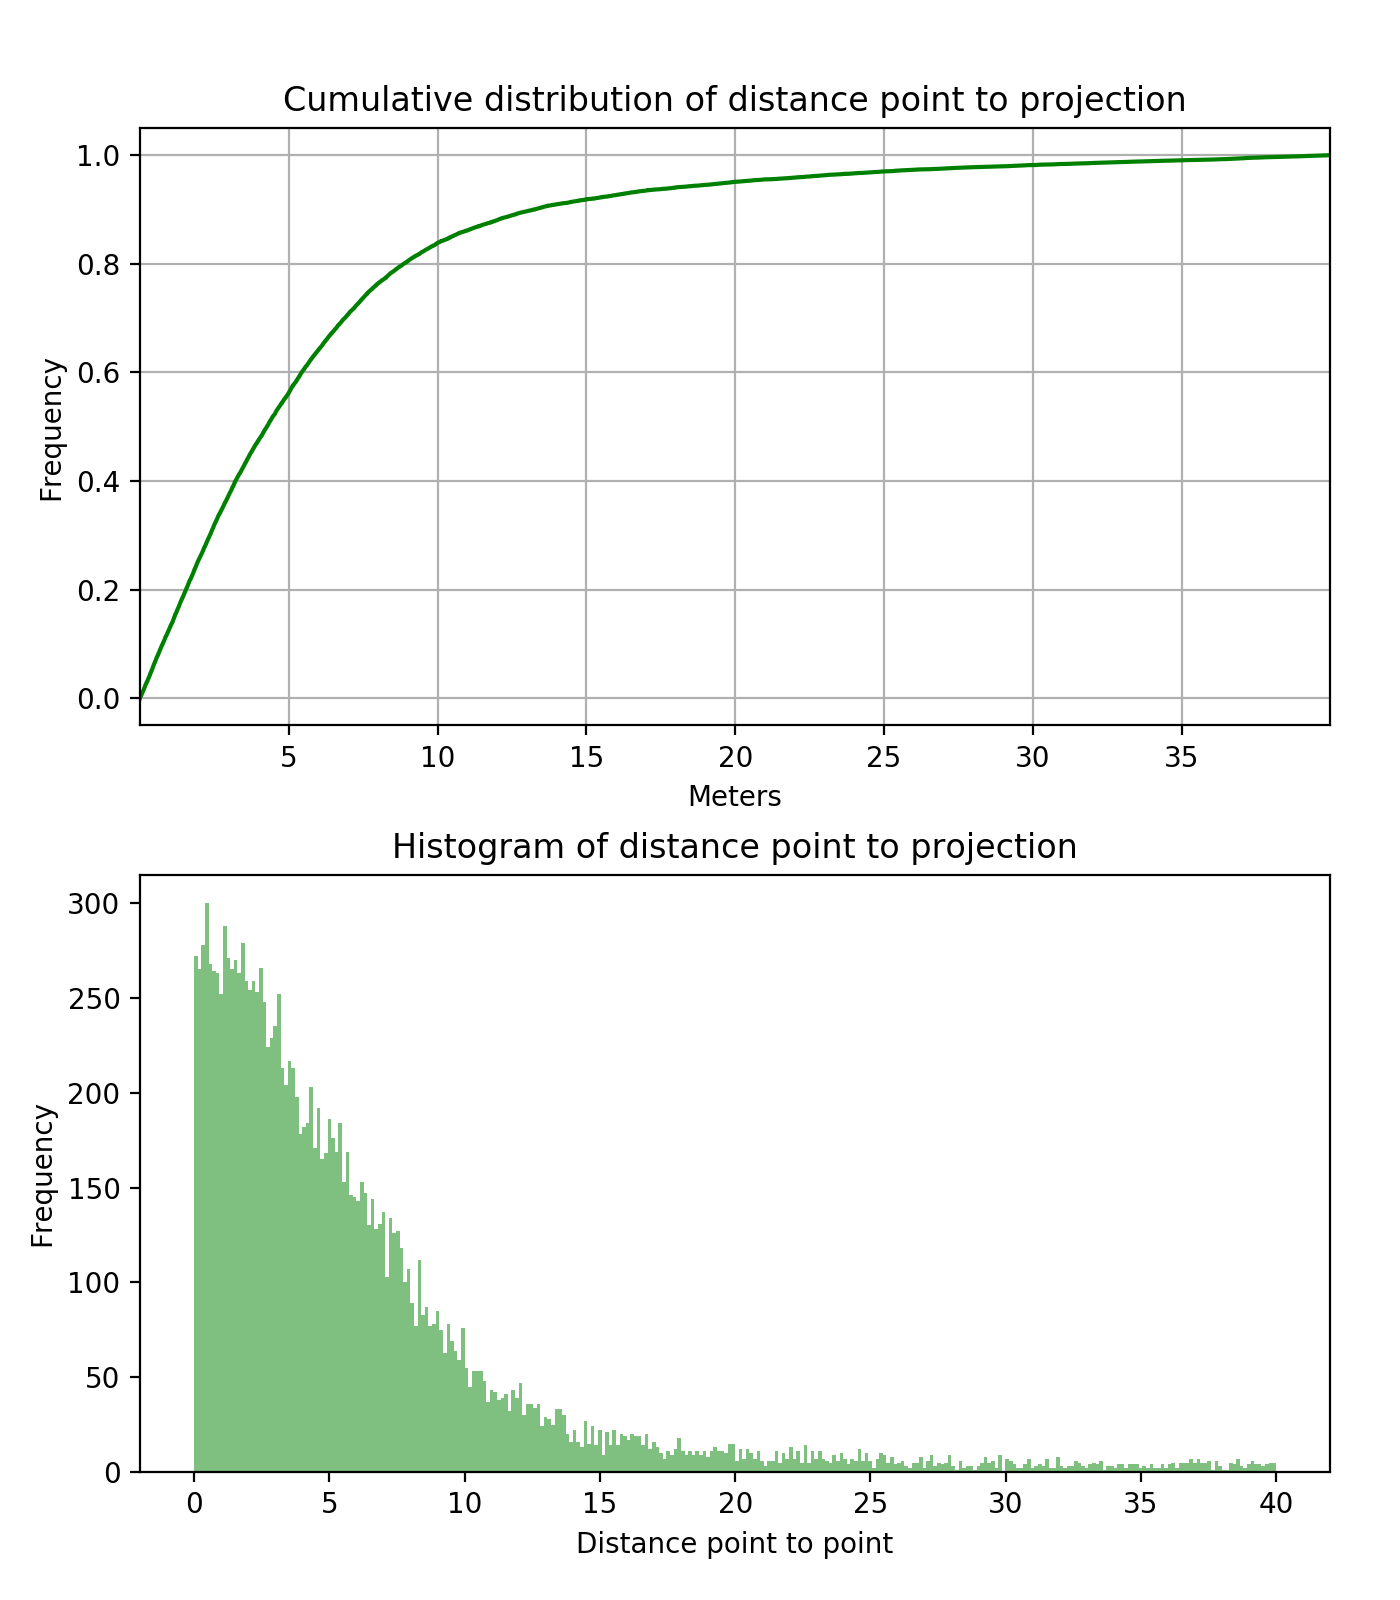
\includegraphics[width=1.2\textwidth]{./Imagenes/PointToProjection.png}
\caption{Análisis de la distancia punto a proyección.}
\label{figure:PointToProjection}
\end{minipage}\hfill
\begin{minipage}{0.48\textwidth}
\centering
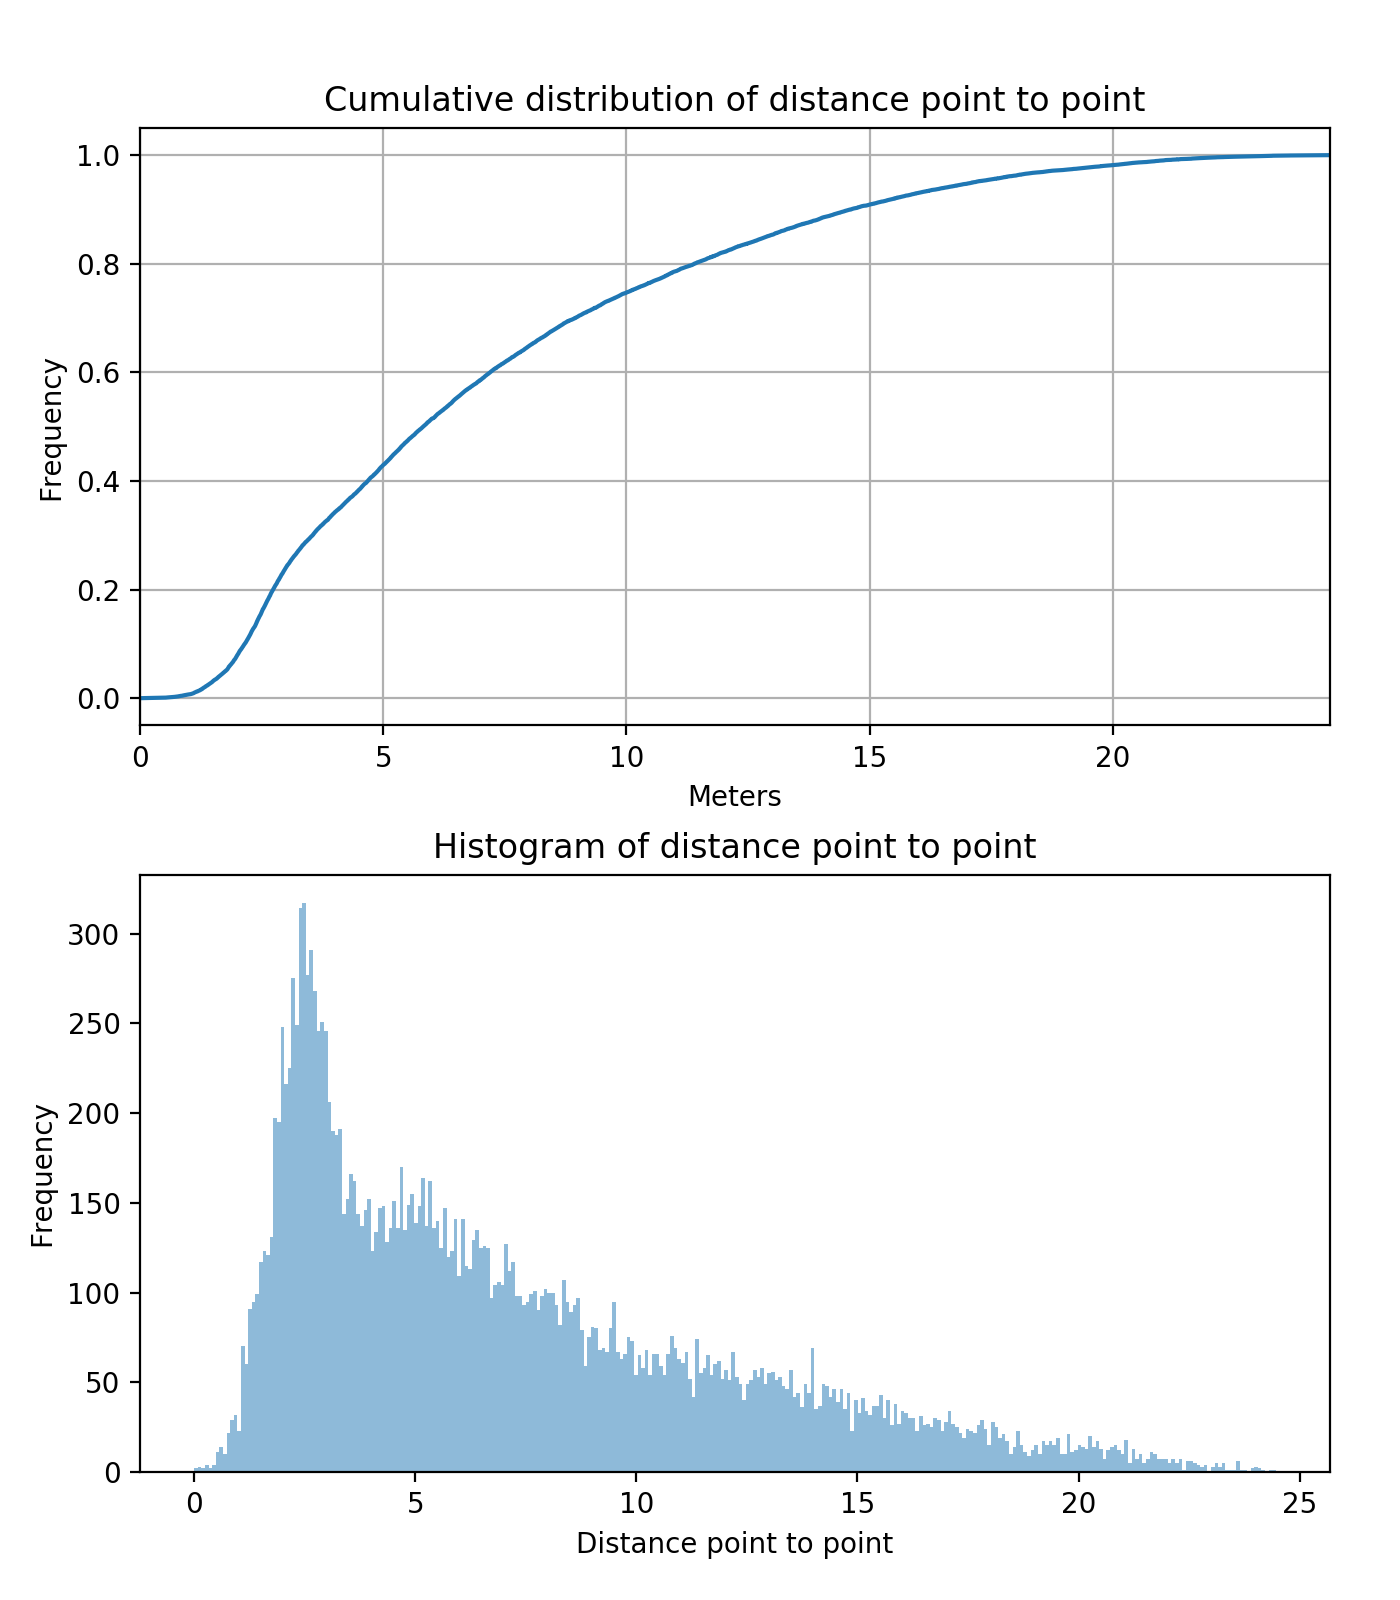
\includegraphics[width=1.2\textwidth]{./Imagenes/PointToPoint.png}
\caption{Análisis de la distancia punto a punto.}
\label{figure:PointToPoint}
\end{minipage}
\end{figure}
\pagebreak

Como se ve en la imagen \ref{figure:PointToProjection} el 80\% de la distancia entre el punto y la 
proyección con el camino correcto está establecido entre 0 y 10 metros de distancia.

En la figura \ref{figure:PointToPoint} vemos la información correspondiente a la distancia 
entre un punto $x_{n}$ y el punto $x_{n+1}$. El espectro de distancia en este caso es mayor, 
esto puede  ser debido  tanto a la frecuencia del dispositivo, como a la velocidad de individuo, que puede variar en función de la pendiente del camino.